% Document
\documentclass[fontsize=8pt,paper=a4,paper=landscape,DIV=calc,]{scrartcl}
\usepackage[T1]{fontenc}
\usepackage{noto}
\usepackage[nswissgerman,english]{babel}
\renewcommand{\familydefault}{\sfdefault}

% Format
\usepackage[top=5mm,bottom=1mm,left=5mm,right=5mm,includehead]{geometry}
\setlength{\headheight}{\baselineskip}
\setlength{\headsep}{0mm}

\usepackage{multicol}
\setlength{\columnsep}{2mm}
\setlength{\columnseprule}{0.1pt}

% Color
\usepackage[svgnames]{xcolor}

% Math
\usepackage{amsmath}
\usepackage{amssymb}
\usepackage{amsfonts}
\newcommand*{\eq}{=}

%% Venn Diagrams
\usepackage{venndiagram}

%% Trees
%%% https://tex.stackexchange.com/a/425271
\usepackage{forest}
\forestset{
    ptree/.style={
        for tree={
            % grow'=0,
            % parent anchor=children,
            % child anchor=parent,
            grow'=east,
            parent anchor=east,
            child anchor=west,
            text width=7mm
        },
        before typesetting nodes={
            for tree={
                split option={content}{:}{content, my edge label},
            },
        },
    },
    my edge label/.style={
        if={
            > O_= {n'}{1}
        }{
            edge label={node [midway, below left, font=\tiny] {#1} }
        }{
            edge label={node [midway, above left, font=\tiny] {#1} }
        },
    }
}

% Code
\usepackage{listings}

\definecolor{ocherCode}{rgb}{1, 0.5, 0} % #FF7F00 -> rgb(239, 169, 0)
\definecolor{blueCode}{rgb}{0, 0, 0.93} % #0000EE -> rgb(0, 0, 238)
\definecolor{greenCode}{rgb}{0, 0.6, 0} % #009900 -> rgb(0, 153, 0)
\definecolor{teal}{rgb}{0.0, 0.5, 0.5}

\lstdefinestyle{code}{
    identifierstyle=\color{black},
    keywordstyle=\color{blue}\bfseries\small,
    ndkeywordstyle=\color{greenCode}\bfseries\small,
    stringstyle=\color{ocherCode}\ttfamily\small,
    commentstyle=\color{teal}\ttfamily\textit\small,
    basicstyle=\ttfamily\small,
    breakatwhitespace=false,
    breaklines=true,
    captionpos=b,
    keepspaces=true,
    showspaces=false,
    showstringspaces=false,
    showtabs=false,
    tabsize=2,
    belowskip=0pt,
    aboveskip=0pt
}

\lstset{
   extendedchars=true,
   basicstyle=\footnotesize\ttfamily,
   tabsize=2,
   breaklines=true,
   showspaces=false,
   showtabs=false
   showstringspaces=false,
   style=code
}

%% https://tex.stackexchange.com/a/536018
%% Allow for German characters in lstlistings.
\lstset{literate=
    {Ö}{{\"O}}1
    {Ä}{{\"A}}1
    {Ü}{{\"U}}1
    {ü}{{\"u}}1
    {ä}{{\"a}}1
    {ö}{{\"o}}1
}

%% Easier inline code
\newcommand{\cinline}[1]{\lstinline[language=c]|#1|}
\newcommand{\jinline}[1]{\lstinline[language=java]|#1|}
\newcommand{\csinline}[1]{\lstinline[language={[Sharp]C}]|#1|}

% Images
\usepackage{graphicx}
\graphicspath{{graphics/}}

% Links
\usepackage{hyperref}
\hypersetup{
    colorlinks=true,
    linkcolor=blue,
    filecolor=magenta,
    urlcolor=cyan,
}

% Smaller Lists
\usepackage{enumitem}
\setlist[itemize,enumerate]{leftmargin=3mm, labelindent=0mm, labelwidth=1mm, labelsep=1mm, nosep}
\setlist[description]{leftmargin=0mm, nosep}
\setlength{\parindent}{0cm}

% Smaller Titles
\usepackage[explicit]{titlesec}

%% Color Boxes
\newcommand{\sectioncolor}[1]{\colorbox{black!60}{\parbox{0.97\linewidth}{\color{white}#1}}}
\newcommand{\subsectioncolor}[1]{\colorbox{black!50}{\parbox{0.97\linewidth}{\color{white}#1}}}
\newcommand{\subsubsectioncolor}[1]{\colorbox{black!40}{\parbox{0.97\linewidth}{\color{white}#1}}}
\newcommand{\paragraphcolor}[1]{\colorbox{black!30}{\parbox{0.97\linewidth}{\color{white}#1}}}
\newcommand{\subparagraphcolor}[1]{\colorbox{black!20}{\parbox{0.97\linewidth}{\color{white}#1}}}

%% Title Format
\titleformat{\section}{\vspace{0.5mm}\bfseries}{}{0mm}{\sectioncolor{\thesection.~#1}}[{\vspace{0.5mm}}]
\titleformat{\subsection}{\vspace{0.5mm}\bfseries}{}{0mm}{\subsectioncolor{\thesubsection~#1}}[{\vspace{0.5mm}}]
\titleformat{\subsubsection}{\vspace{0.5mm}\bfseries}{}{0mm}{\subsubsectioncolor{\thesubsubsection~#1}}[{\vspace{0.5mm}}]
\titleformat{\paragraph}{\vspace{0.5mm}\bfseries}{}{0mm}{\paragraphcolor{\theparagraph~#1}}[{\vspace{0.5mm}}]
\titleformat{\subparagraph}{\vspace{0.5mm}\bfseries}{}{0mm}{\subparagraphcolor{\thesubparagraph~#1}}[{\vspace{0.5mm}}]

%% Title Spacing
\titlespacing{\section}{0mm}{0mm}{0mm}
\titlespacing{\subsection}{0mm}{0mm}{0mm}
\titlespacing{\subsubsection}{0mm}{0mm}{0mm}
\titlespacing{\paragraph}{0mm}{0mm}{0mm}
\titlespacing{\subparagraph}{0mm}{0mm}{0mm}

%define header and footer
\usepackage{fancyhdr}
\pagestyle{fancy}

\fancyhead[RO]{\AUTHOR\hspace{4pt}|\hspace{4pt}\INSTITUTE}
\fancyhead[LO]{\TITLE}
\usepackage[style=iso]{datetime2}
\fancyfoot[RO]{\today}
\renewcommand\headrulewidth{0pt}
\renewcommand\footrulewidth{0pt}
\headsep = -2pt
\footskip = 0pt

% no vertical distribution
%% explanation: we copy the macro columnbreak to stdcolumnbreak
%% we now redefine columnbreak to always fill up null space and then execute the standard columnbreak.
\let\stdcolumnbreak\columnbreak
\renewcommand\columnbreak{\vfill\null\stdcolumnbreak}


\newcommand{\TITLE}{Parallel Programming}
\newcommand{\AUTHOR}{Mona Panchaud}
\newcommand{\INSTITUTE}{Ostschweizer Fachhochschule}

\begin{document}
\begin{multicols*}{4}

\section{Java Threads}
    \begin{lstlisting}[language=java]
public static void main(String[] args) {
    var a = new Thread(() -> multiPrint("A"));
    var b = new Thread(() -> multiPrint("B"));
    a.start(); // here we start the thread!
    b.start();
    System.out.println("main finished");
}
\end{lstlisting}

\section{Java Monitor}
    Impossible for two invocations of \textbf{synchronized} methods on the same object to interleave.\\
    Possible Fairness-Problem with \jinline{notify()}/\jinline{notifyAll()}
    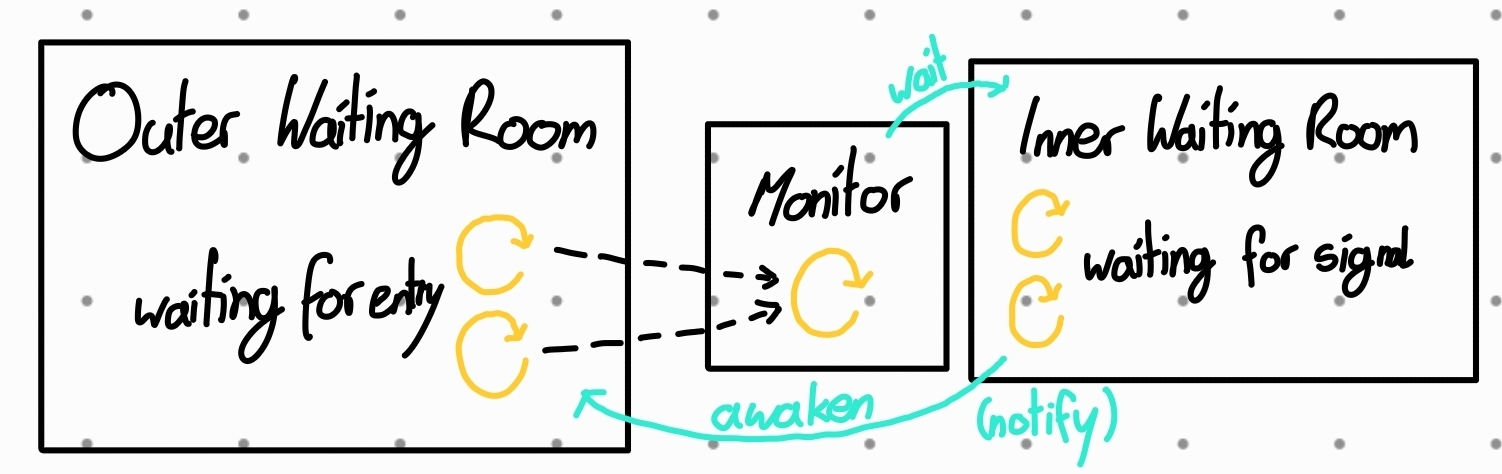
\includegraphics[width=0.2\textwidth]{monitor}
    \subsection{Monitor ``Traps''}
        \begin{itemize}
            \item \jinline{notify()} wakes up random thread. Doesn't work if we have different conditions waited upon
            \item Awakened thread must retry to get monitor and can be overtaken. Wait with \jinline{while} loop instead of \jinline{if}.
        \end{itemize}

    % TODO maybe throw one of those examples out dependent on space?
    \subsection{Queue Example}
    \begin{lstlisting}[language=java]
public synchronized void put(T x) throws InterruptedException {
    while (queue.size() == capacity) {
        wait(); // await non-full
    }
    queue.add(x);
    notifyAll(); // signal non-empty
}
public synchronized T get() throws InterruptedException {
    while (queue.size() == 0) {
        wait(); // await non-empty
    }
    T x = queue.remove();
    notifyAll(); // signal non-full
    return x;
}
\end{lstlisting}

    \subsection{Barrier Example}
    \begin{lstlisting}[language=java]
public synchronized void waitForParticipants() throws InterruptedException {
  arrived++;
  if (arrived == participants) {
    notifyAll();
  }
  while (arrived < participants) {
    wait();
  }
}
\end{lstlisting}

\section{Specific Synchronization Mechanisms}
    \subsection{Semaphore}
    Thread that releases permit doesn't need to have acquired that permit by calling acquire().\\
    acquire() \jinline{throws InterruptedException}

    Pattern:
    \jinline{x.acquire(); try \{ y.acquire() \} finally \{ x.release() \}})
    \subsection{ReentrantLock}
    Only thread that acquired lock can unlock.

    Condition replaces use of Object monitor methods.
    \begin{lstlisting}[language=java]
Lock monitor = new ReentrantLock(true);
Condition nonFull = monitor.newCondition();
nonFull.await(); nonFull.signal();
\end{lstlisting}

    \subsection{ReentrantReadWriteLock}
    If write access involved: acquire write lock! (also if only conditionally)

    Conditions only supported on write-locks

    \subsection{CountDownLatch}
    Counter until 0. ``Tür geht auf'' \& bleibt offen.
    % TODO maybe remove because of space reasons?
    \begin{lstlisting}[language=java]
var ready = new CountDownLatch(N);
ready.countDown(); ready.await();
\end{lstlisting}

    \subsection{CyclicBarrier}
    Like Latch but reusable $\Rightarrow$ (Tür geht auch wieder zu)
    % TODO maybe remove because of space reasons?
    \begin{lstlisting}[language=java]
var gameRound = new CyclicBarrier(N);
gameRound.await();
\end{lstlisting}

    \subsection{Rendez-Vous}
    Two threads meet and exchange object
    \begin{lstlisting}[language=java]
var exchanger = new Exchanger<Integer>();
int out = exchanger.exchange(myInt);
\end{lstlisting}

\section{Java Thread Pool}
	Tasks are queued into Queue. There are worker threads (daemon) that grab tasks from the queue and execute them. Any task must complete before worker thread can grab another task. As it is daemon we need to ensure that main thread is not done earlier than the tasks in the queue.

    \begin{lstlisting}[language=java]
var threadPool = new ForkJoinPool();
ForkJoinPool.commonPool(); // Singleton. Doesn't always use all processors
Future<T> future = threadPool.submit(...); // launches task async, doesn't block
T res = future.get();// blocks until terminated
Future<Integer> future = threadPool.submit(() -> {
    int value = ...;
    // long calculation
    return value;
}); // put task into pool, doesn't block
\end{lstlisting}
    We should avoid over parallelization! Therefore use a threshold.

    % TODO maybe remove one of the examples because of space reasons?
    \subsection{Fork/Join Example 1}
    \begin{lstlisting}[language=java]
// Need to extend when we want to use fork!
// When no return value: Use RecursiveAction
class CountTask extends RecursiveTask<Integer> {
  private final int lower, upper;
  public CountTask(int lower, int upper) {
    this.lower = lower; this.upper = upper;
  }
  protected Integer compute() {
    if (lower == upper) { return 0; }
    if (lower + 1 == upper) { return isPrime(lower) ? 1 : 0; }
    int middle = (lower + upper) / 2;
    var left = new CountTask(lower, middle);
    var right = new CountTask(middle, upper);
    left.fork(); right.fork();
    return right.join() + left.join();
  }
}
\end{lstlisting}

    \subsection{Fork/Join Example 2 with invokeAll}
    \jinline{invokeAll(a, b)} equivalent to \jinline{a.fork(); b.fork(); b.join(); a.join();}
    \begin{lstlisting}[language=java]
protected void compute() {
  if (rowRight - rowLeft > THRESHOLD) {
    var middle = (rowLeft + rowRight) / 2;
    invokeAll(
      new MatrixFillTask(array, rowLeft, middle, colLeft, colRight),
      new MatrixFillTask(array, middle, rowRight, colLeft, colRight));
  } else if (colRight - colLeft > THRESHOLD) {
    var middle = (colLeft + colRight) / 2;
    invokeAll(
      new MatrixFillTask(array, rowLeft, rowRight, colLeft, middle),
      new MatrixFillTask(array, rowLeft, rowRight, middle, colRight));
  } else {
    for (int row=rowLeft; row<rowRight; row++) {
      for (int col=colLeft; col<colRight; col++) {
        array[row][col] = (row + 1) * (col + 1);
      }
    }
  }
} // ...
threadPool.invoke(new MatrixFillTask(matrix, 0, matrix.length, 0, matrix[0].length));
\end{lstlisting}


\section{C\# Parallelization}
    Lots of quickly iterating bodies is inefficient.
    Therefore TPL automatically groups multiple bodies into a single task.
    \subsection{C\# Parallel Examples}
    \begin{lstlisting}[language={[Sharp]C}]
var task = Task.Run(() => {
  var left = Task.Run(() => Count(leftPart));
  var right = Task.Run(() => Count(rightPart));
  return left.Result + right.Result;
});
static Task<int> Count(... part) { ... }

Parallel.Invoke(
  () => MergeSort(l, m),
  () => MergeSort(m, r)
);

Parallel.ForEach(list, file => Convert(file));

Parallel.For(0, dimN, i => {
  Parallel.For(0, dimM, j => {
    matrixC[i, j] = 0;
    for (var k = 0; k < dimK; k++) {
      matrixC[i, j] += matrixA[i, k] * matrixB[k, j];
    }
  });
});

bookCollection.AsParallel()
  .Where(book => book.Title.Contains("Title"))
  .Select(book => book.ISBN);
\end{lstlisting}

\section{Data Race \& Race Condition}
    \subsection{Data Race}
    \begin{itemize}
        \item $\geq$ 2 threads in a \textbf{single process} access the same memory location concurrently
        \item \& at least one of the accesses is for writing
        \item \& not using any exclusive locks
    \end{itemize}

    \subsection{Race Condition}
    \begin{itemize}
        \item Multiple threads access shared resources without \textbf{sufficient} synchronization
        \item Cause is often Data Race but not always. Can also be a lack of synchronization over larger blocks.
    \end{itemize}

	\begin{lstlisting}[language=java]
private volatile boolean locked = false;
public void acquire() {
	// these two operations would need to be atomar, otherwise there's a race condition
	while (locked) {}
	locked = true;
} // -> use AtomicBoolean and while(myBool.getAndSet(true)) {}
\end{lstlisting}

    \subsection{Deadlock}
    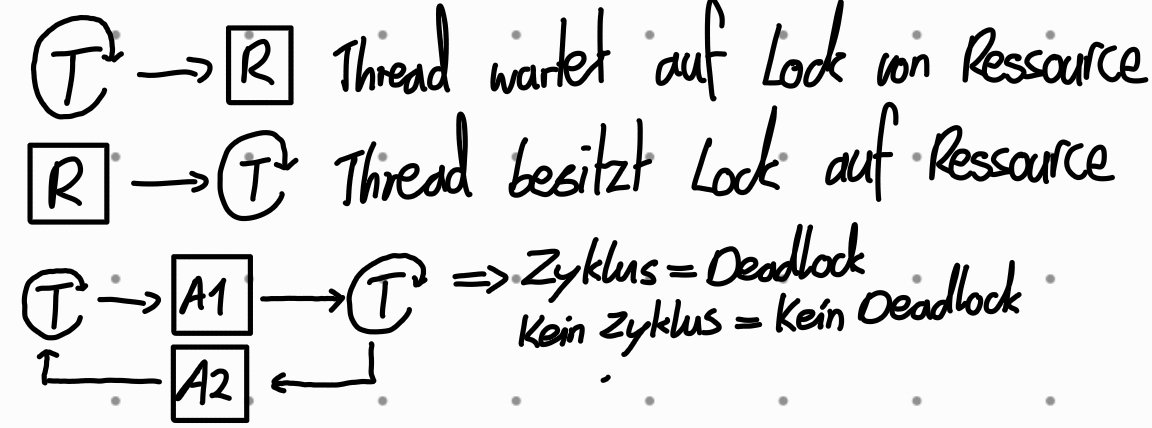
\includegraphics[width=0.15\textwidth]{deadlock_detection}
    \begin{description}
        \item[Livelock] Deadlock. But still use CPU (e.g. \jinline{while} loop)
    \end{description}

    \begin{lstlisting}[language=java]
// Synchronized locks can get nested:
synchronized void transfer(MySemaphore o) {
    o.release(count); }
synchronized void release(int amount) { ... }
// Which can lead to Deadlock.
// Possible Scenario:
s1.transfer(s2);
s2.transfer(s1);
\end{lstlisting}
    \subsubsection{Avoidance}
        \begin{itemize}
            \item Linear locking order. (e.g. only ascending)
            \item Grobgranulare locks (e.g. lock whole bank at account access)
        \end{itemize}

\section{asynchronous Programming}
\begin{description}
	\item[Caller centric (pull)] Caller waits for task and gets result
	\item[Callee centric (push)] Task hands over result directly to successor
\end{description}

\begin{lstlisting}[language={[Sharp]C}]
Task.Run(task1).ContinueWith(task2);
Task.WhenAll(task1, task2).ContinueWith(task3);
Task.WhenAny(task1, task2).ContinueWith(task3);
\end{lstlisting}
C\# \textit{Exceptions} in Fire \& Forget Tasks are ignored. (wait at end, but if exc in task1 \& only waited for task2 exc is still ignored or use TaskScheduler.UnobservedTaskException. Both depend on GarbageCollection.)

\begin{lstlisting}[language=java]
CompletableFuture.supplyAsync(() -> firstOp)
	.thenApplyAsync(two).thenAcceptAsync(three);
\end{lstlisting}
\textbf{Mit Return:} \jinline{supply} (async call), \jinline{thenApply} (continuation)
\textbf{void:} \jinline{run} (async call), \jinline{thenAccept} (continuation)

\textbf{Exception Handling}: \jinline{exceptionally()} in task chain, only run chain until next exceptionally

\subsection{GUI Thread Modell}
\underline{Only} \textbf{UI Thread} is allowed to access UI components

$\Rightarrow$ In C\# Exception, in Java Race Condition.

No long operations in UI thread, otherwise UI blocked.

C\# \csinline{Dispatcher.InvokeAsync} but better to use \csinline{await} (if await is done in UI Thread the Continuation is dispatched from Worker thread to UI thread),\\
Java: \jinline{SwingUtilities.invokeLater}

\section{Volatile / Visibility / Atomic Operations}
	\textit{Weak Memory Model}: Memory accesses are seen in different order by different threads

	\textit{Atomicity} doesn't mean visibility (order: unlock -> lock, volatile write -> volatile read)

    \begin{minipage}[c]{.6\linewidth}
        \textbf{Java}:
        \begin{itemize}
            \item data types until 32 bit atomar operations
            \item 64 bit with volatile keyword atomar
        	\item partial order given by visibility
            \item volatile is not reordered (total order)
        \end{itemize}
    \end{minipage}%
    \begin{minipage}[c]{.1\textwidth}
        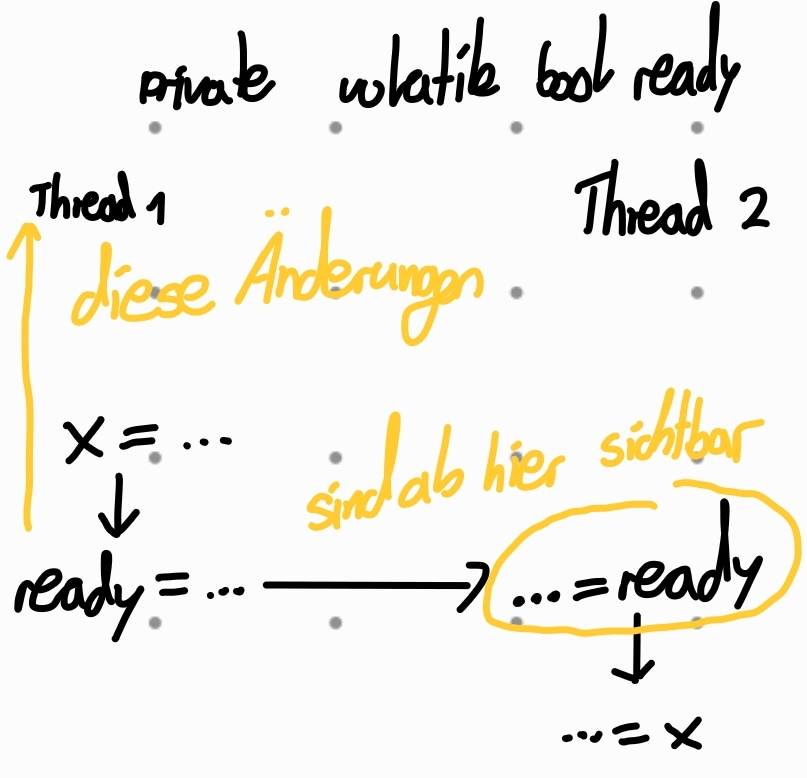
\includegraphics[width=\linewidth]{volatile_visibility}
    \end{minipage}%
    \\ % <- important so that C# is still displayed!
    \textbf{C\#}:
    \begin{itemize}
        \item volatile long/double not atomar
        \item visibility is given when ordering is given
        \item only partial order: everything before volatile write stays before.
        \item everything after volatile read stays afer
        \item Full Fence with \csinline{Thread.MemoryBarrier()}
    \end{itemize}

    \subsection{compareAndSet}
    In one atomic operation (hardware support):
    \begin{lstlisting}[language=java]
if (current == expect) {
    current = update;
    return true;
} else {
    return false;
}
\end{lstlisting}

    Trick for more atomic operations (like \jinline{updateAndGet})
    (Write, only in case the read value is still the same)
    \begin{lstlisting}[language=java]
do {
    oldVal = var.get();
    newVal = calculateChanges(oldVal);
} while (!var.compareAndSet(oldVal, newVal));
\end{lstlisting}

\section{CUDA}
We want compute bound applications for GPU!

	\subsection{General Terms}
	\begin{description}
		\item[Latency] 	how long does it max. take to execute an instruction/operation
		\item[Troughput] 	instructions or operations completed per second
		\item[Compute bound] compute time is longer
		\item[Memory bound] memory time is longer
		\item[Arithmetic intensity] \(\frac{\text{number of operations}}{\text{number of transferred bytes}}\)
	\end{description}
	\textbf{Pipelining} \\ 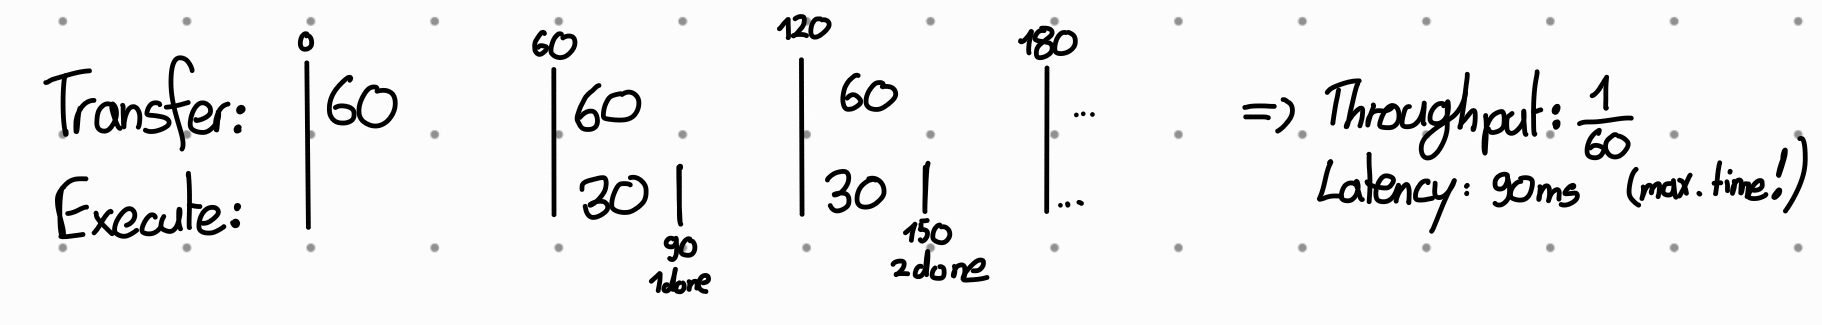
\includegraphics[width=0.25\textwidth]{latency_throughput}

	\subsection{Guarantees}
	\begin{enumerate}
		\item all threads in block run on \textbf{same} SM at same time
		\item Blocks in kernel finish before any block from new kernel can be started
	\end{enumerate}

	\subsection{Memory Model}
	\begin{itemize}
		\item shared memory (fast): visible to all threads in a block
		\item global memory (slow): visible to all threads
		\item local memory (slow): private to thread
		\item unified memory: memory accessible from CPU \& GPU
	\end{itemize}
	\cinline{syncthreads();} synchronize all threads in block. (e.g. before loading new shared memory)

    \textbf{shared memory} useful when multiple threads use the same memory

	\subsection{Number of Threads per Block}
Maximum threads per block: 1024

Max thread dimension per block	(1024, 1024, 64)

We can allocate \textbf{at most} 1024 threads in one block, in the specified dimensions.
i.e. \cinline{dim3(32, 32, 1)} or \lstinline[language=c]|dim3(16, 16, 4)| or just 1024.

	\subsection{2D Grid Blocks}
	For 200x900 image: \lstinline[language=c]|dim3(32, 32, 1)| (block size)
	ceil(200/32) x ceil(900/32) $\rightarrow$ \lstinline[language=c]|dim3(7, 29, 1)| (grid)

	\subsection{Warps}
	Threads with the same instruction $\Rightarrow$ grouped into warps.
	Several Warps $\Rightarrow$ thread block.

	Several thread blocks $\Rightarrow$ to Streaming Multiprocessor.

	\subsection{Thread Divergence}
	When there's a thread \textbf{in the same warp}:
	\begin{enumerate}
		\item execute one branch, other threads need to wait
		\item execute other branch, other threads need to wait
	\end{enumerate}
	Avoid with e.g: \cinline{if(threadIdx.x / 32 > 1) \{ ... \}}

	Figure out how many warps have \textbf{thread divergence}: Figure out how many warps execute different branches in different threads.

	\subsection{Memory Coalescing}
	Threads should access 32-byte areas (dependent on memory bus size => 256 bit = 32 byte) we can profit from burst read.

	\begin{lstlisting}[language=c]
data[(Expression without threadIdx.x) + threadIdx.x]
\end{lstlisting}

	\subsection{Vector Add Example}
	\begin{lstlisting}[language=c]
__global__
void cudaVectorAdd(float *a, float *b, float *c, int numElements) {
  int i = blockDim.x * blockIdx.x + threadIdx.x;
  if(i < numElements) {
    c[i] = a[i] + b[i];
  }
}
// main
size_t size = N * sizeof(float);
float *d_a, *d_b, *d_c;
// wrap with "handleCudaError"
cudaMalloc(&d_a, size);
cudaMalloc(&d_b, size);
cudaMalloc(&d_c, size);
cudaMemcpy(d_a, h_a, size, cudaMemcpyHostToDevice);
cudaMemcpy(d_b, h_b, size, cudaMemcpyHostToDevice);

int threadsPerBlock = 1024;
int blocksInGrid = (N + threadsPerBlock - 1) / threadsPerBlock;
// make sure to pass in d_ variables!
cudaVectorAdd<<<blocksInGrid,threadsPerBlock>>>(d_a, d_b, d_c, N);
cudaMemcpy(h_c, d_c, size, cudaMemcpyDeviceToHost);
// cudaFree, free
\end{lstlisting}

\subsection{2D to 1D Example}
\begin{lstlisting}[language=c]
int row = blockIdx.x * blockDim.x + threadIdx.x
int col = blockIdx.y * blockDim.y + threadIdx.y
elements[row * COLS + col] = whatever;
\end{lstlisting}

\section{MPI}
MPI\_Reduce: MPI\_MAX,MPI\_MIN,MPI\_SUM,MPI\_PROD

    \begin{lstlisting}[language=c]
MPI_Init(&argc, &argv);
int rank, size;
MPI_Comm_rank(MPI_COMM_WORLD, &rank);
MPI_Comm_size(MPI_COMM_WORLD, &size);
int amountOfRows = (IMAGE_HEIGHT + size - 1) / size; // ceil
if(rank == 0) {
	for (int from = 1; from < size; from++) {
		MPI_Recv(arrayPtr, sizeofArray, MPI_INT, from, 0, MPI_COMM_WORLD, MPI_STATUS_IGNORE);
	}
} else {
	MPI_Send(arrayPtr, amountOfRows * IMAGE_WIDTH, MPI_INT, toWhichProcess, 0, MPI_COMM_WORLD);
}
MPI_Finalize();
\end{lstlisting}
    \subsection{MPI Find Max Int in Array Example}
    \begin{lstlisting}[language=c]
int length;
if (rank == 0) {
  array = read_array_file(&length);
  int partition = length / size;
  for (int to = 1; to < size; to++) {
    int offset = rank * partition;
    if (to == size - 1) { partition = length - offset; }
    MPI_Send(&partition, 1, MPI_INT, to, 0, MPI_COMM_WORLD);
    MPI_Send(array + offset, partition, MPI_INT, to, 0, MPI_COMM_WORLD);
  }
  if (size > 1) {
    length = partition;
  }
} else {
  MPI_Recv(&length, 1, MPI_INT, 0, 0, MPI_COMM_WORLD, MPI_STATUS_IGNORE);
  MPI_Recv(array, length, MPI_INT, 0, 0, MPI_COMM_WORLD, MPI_STATUS_IGNORE);
} // what follows is the sequential code:
int maximum = INT_MIN;
for (int i = 0; i < length; i++) {
  if (array[i] > maximum) {
    maximum = array[i];
  }
} // reduce to one value:
int result;
// third param: count, second last: root
MPI_Reduce(&maximum, &result, 1, MPI_INT, MPI_MAX, 0, MPI_COMM_WORLD);
printf("maximum: %i", result);
\end{lstlisting}%

\section{Performance Analysis}
Parallelization overhead ignored by both laws.
\subsection{Amdahls Law}
Problem size doesn't change
$\rightarrow$ Strong Scaling

\begin{minipage}{0.08\textwidth}
    \(speed up = \frac{1}{s + \frac{p}{N}}\)
\end{minipage}
\begin{minipage}{0.9\textwidth}
    \begin{description}
        \item[s] serial part
        \item[p] part that we can parallelize
        \item[N] processor count
    \end{description}
\end{minipage}

\subsection{Gustafson's Scaling}
Problem size \& no. of processors increases
$\rightarrow$ Weak Scaling.
\(speed up = s + p * N = s + (1-s) * N \)

\subsection{Roofline Model}
% TODO Bildli auf gedrucktes Blatt zeichnen

$\pi$ = max performance, $\beta$ = Bandwidth, I = Arithmetic Intensity

Ridge point is at \(I = \frac{\pi}{\beta}\)

Max. Attainable Performance: \(min(\pi, \beta * I)\) in (flops/s)

At which arithmetic intensity processor 2 becomes faster than processor 1: \(\frac{\pi_1}{\beta_2}\)

\section{OpenMP}
Depend on previous values: Read Write Dependency
	\begin{lstlisting}[language=c]
int A, B;
#pragma omp parallel for private (A)
// Each thread processes one iteration at a time. Each thread has private copy of A. B is shared.

int i;
#pragma omp parallel for
	for(i = 0; i < N; i ++) {}
// Loop iterator is private but only when using omp loop constructs!!

#pragma omp critical { /*critical section*/ }
// Heavy weight mutex => large performance overhead
// Lightweight mutex with atomic (but limited)
\end{lstlisting}

\end{multicols*}
\end{document}